\chapter{Ingegneria dei requisiti}
\section{Requisiti}
Il requisito è la descrizione delle funzionalità di un sistema software,
nella condizione in cui questo sistema dovrebbe funzionare. Riflette le 
necessità del cliente e le sue aspettative su software. Sembra semplice, ma 
è critico.

\subsection{User requirements}
Parliamo dei user requirements, ovvero i requisiti utente. Questi sono
requisiti ad alto livello, date dall'utente che esprimono il comportamento del sistema,
sono tipicamente frase astratte e generiche, non prevedono una soluzione.
Tipicamente scritti con il cliente.

\subsection{System requirements}
System requirements, ovvero i requisiti di sistema, sono requisiti più specifici,
strutturati e formali. Tipicamente si va nel dettaglio, comprensibile anche 
dall'utente.
I requisiti di sistema possono essere utili per l'utente per essere validati.

\section{Stakeholders}
Tutte le persone coinvolte nel progetto,
che hanno un interesse nel progetto. Quindi utenti e tutti quelli che verranno 
toccati dal sistema software.

\section{Requisiti funzionali e non funzionali}
\subsection{Requisiti funzionali}
Quando parliamo di requisiti funzionali intendiamo requisiti che catturano 
funzionalità che il sistema deve fornire. Raccoglie scenari, come deve agire, 
come agisce, cosa fa, cosa non fa.

Ci sono diversi livelli di astrazione, alcuni descrivono l'alto livello.

Possono essere ambigui. Bisogna segnalare l'ambiguità per evitare errori.

Devo raggiungere l'obiettivo della completezza, ovvero che tutte le funzionalità devono essere 
catturate dai miei requisiti. Il secondo obiettivo è la consistenza, ovvero che non 
devono essere alterati.

In pratica questi due obiettivi nella realtà non vengono mai raggiunti al 100\%, quindi 
potrebbero esserci incomprensioni tra stakeholder.
Alcuni problemi emergono in fase di sviluppo.
\subsection{Requisiti non funzionali}
Descrivono caratteristiche che non sono funzionalità, ma sono importanti per 
la soddisfazione del cliente. 
Coinvolgono tutti i componenti. Ambienti di sviluppo, standard da soddisfare, performance, 
requisiti di qualità, requisiti di interfaccia.

Richieste che vincolano l'architettura del sistema.
Un requisito non funzionale potrebbe generare più requisiti funzionali.
Non emergono dalla discussione.

Ad esempio i \textbf{requisiti di prodotto}, specificano comportamento
del sistema e si specializza in diversi tipi di requisiti.
\begin{figure}[H]
    \centering
    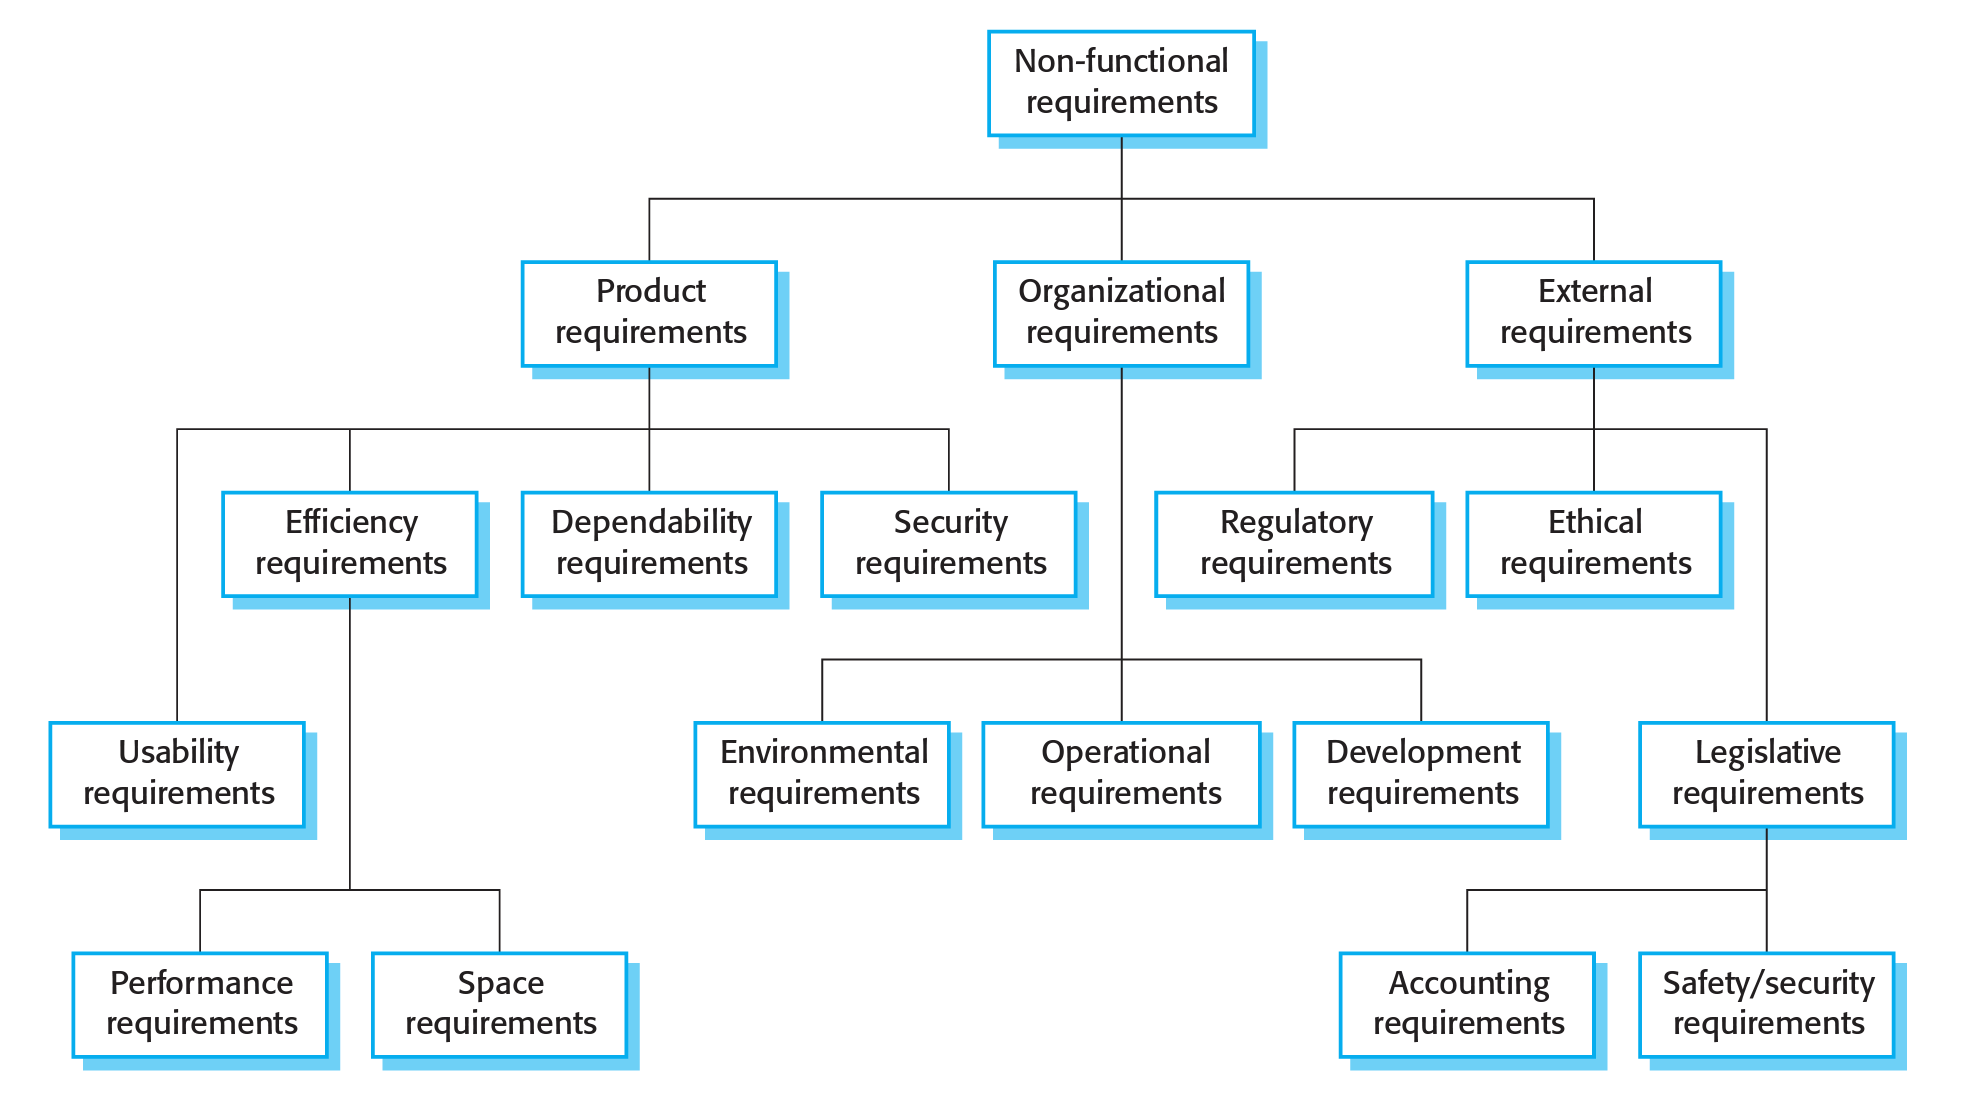
\includegraphics[scale=0.4]{img/nonfunctional.png}
\end{figure}
È opportuno segnalare più requisiti non funzionali, per evitare che vengano 
persi, quindi da qualitativo deve diventare quantitativo.
Riduce la contestazione di un sistema, riducendo il grado di contestabilità, per 
togliere astrazione.

Le metriche per trasformarli in requisiti quantitativi sono:
\begin{itemize}
    \item Velocità;
    \item Dimensione;
    \item Facilità di utilizzo;
    \item Reliability;
    \item Robustezza;
    \item Portabilità;
\end{itemize}
\section{Processi di ingegneria dei requisiti}
Ci sono tre fasi:
\begin{itemize}
    \item Raccolta: ho la descrizione del sistema;
    \item Specifica: ho il documento di specifica dei requisiti;
    \item Validazione: ho il documento di validazione dei requisiti;
\end{itemize}
Ognuna di queste fasi ha un output. In generale la raccolta può essere visto 
come un processo  a spirale.
\begin{figure}[H]
    \centering
    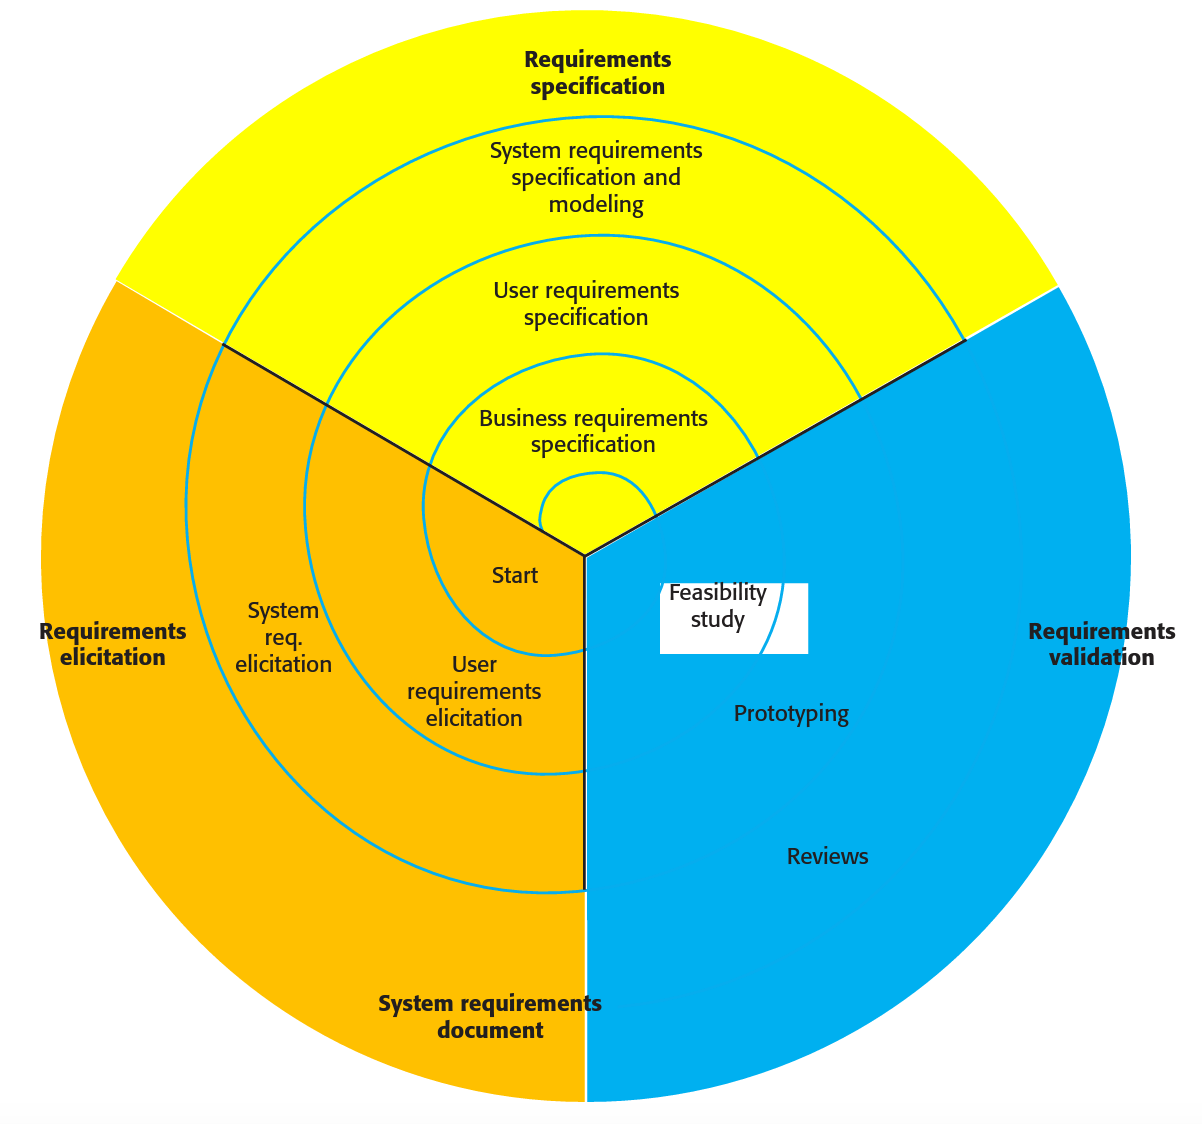
\includegraphics[scale=0.4]{img/spiralerequisiti.png}
\end{figure}
\subsection{Elicitazione dei requisiti}
Devono capire il dominio applicativo, funzionalità che dovrà fornire, 
vincoli non funzionali come le performance, hardware con cui dovrà interagire.
Ci potrebbero essere ostacoli, sistemi non realizzabilit, 
i clienti possono esporre i requisiti con termini non noti 
agli ingegneri del software o sottointendere requisiti per sono ovvi 
nel loro dominio applicativo.

Con differenti stakeholder, si possono avere differenti obiettivi,
quindi potremmo raccogliere requisiti in conflitto tra loro. 
Potrebbero non collaborare se qualcuno non si sente rappresentato.
Potrebbero esserci fattori politici. Potrebbero cambiare nel corso dello 
sviluppo, o emergere. Le esigenze intrinseche del cliente potrebbero.

Il primo modo per raccogliere i requisiti è mediante 
intervista, con risposte chiuse o domande aperte. In genere mista. Gli stakeholders 
non forniscono requisiti dettagliati. Non è semplice condurre un'intervista in 
maniera efficace. 
Cercare di evitare pregiudizzio, prima di portarmi avanti con assunzioni verifico.
Iniziare con domande trampolino, non iniziare con cose molto astratte.

\subsection{Etnografia}
Non intervistare le persone, ma lavorare insieme a loro, per capire il loro
necessità. Questo aiuta molto la conoscenza implicita che potrebbe non emergere 
durante l'intervista. Questo tipo di studio può essere attuato un sistema software, 
o un processo in atto.
\subsection{Storie e scenari}
Sono dei modi concreti per descrivere un esempio reale del sistema software in 
un particolare contesto. Possono essere presentato allo stakeholder che può 
esprimere parere e dire se qualcosa va bene o no.
Le storie sono testi narrativi, ad alto livello, che descrivono un'interazione
e sono facili da comprendere.
Lo scenario è un esempio di utilizzo del sistema, che descrive un'interazione
tra utente e sistema. È più dettagliato e preciso (ho un input specifico).

Una storia raccoglie può quindi raccogliere più scenari.

\subsection{Documento dei requisiti}
È un documento che contiene tutti i requisiti del sistema software.
i requisiti dell'utente devono essere raccolti dall'utente, 
i requisiti di sistema vengono catturati dagli ingegneri del software.

Scrivendo i requisiti emergono anche architetture o magari dalla descrizione 
capiamo che deve operare con altri sistemi. Oppure vincoli da alcuni documenti.

Il primo modo per raccogliere i requisiti è il linguaggio naturale,
che però è intrinsecamente ambiguo. Quindi adoperare un linguaggio formale,
utilizzando i verbi modali in modo corretto. Testi in grassetto per 
evidenziare parti chiave, mediante artefatto topografico.
Tipicamente si inserisce il motivo per cui un requisito è 
necessario. Tipicamente si aggiungono anche identificativi univoci.

Un'altra tecnica è una forma più vincolata. Spesso su sistemi verificati 
da terze parti.

\subsection{Use cases}
L'use case è una descrizione di un insieme di sequenze di azioni che un sistema
e serve per identificare gli attori e le funzionalità del sistema che fanno 
riferimento ai vari utenti.
\begin{figure}[H]
    \centering
    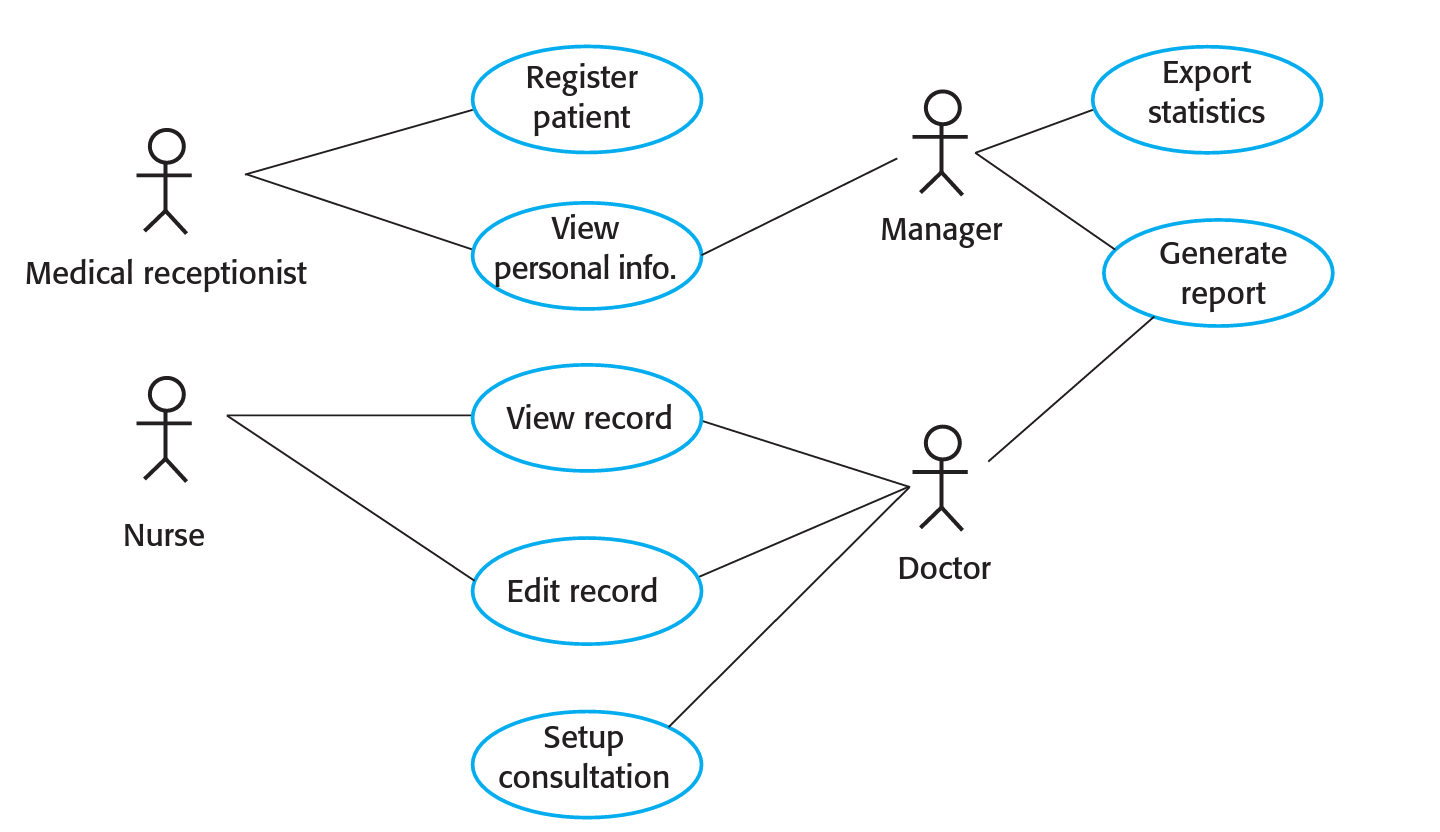
\includegraphics[scale=0.4]{img/usecase.png}
\end{figure}
\subsection{Documento dei requisiti}
Per specificare i requisiti parliamo di documento dei requisiti software.
Può esserci variabilità su questo docomento, ci sono organizzazioni internazionali 
che possono definire standard (esempio IEEE).
\subsubsection{IEEE stuttura}
\begin{itemize}
    \item prefazione
    \item Introduzione 
    \item Glossario: la terminologia è un insieme di keyboard;
    \item Definizione dei requisiti utente;
    \item Vicoli per l'architettura;
    \item Requisiti di sistema;
    \item Modelli di sistema
    \item Evoluzione del sistema;
    \item Appendice;
    \item Indice;
\end{itemize}
Gli utenti interessati sono:
\begin{itemize}
    \item Utenti: chi usa il sistema;
    \item Manager: possono stimare costi e rischi;
    \item Ingegneri del sistema: possono capire cosa devono fare;
    \item Ingegneri del software legati al test: per i test in determinati scenari.
    \item Ingegneri legati alla manutenzione: possono non essere legati al progetto originale;
\end{itemize}
\section{Cambiamento dei requisiti}
Possono evolvere durante lo sviluppo, bisogna dotarsi di un processo. Bisogna analizzare 
il costo che il cambiamento comporta. Tracciare i cambiamenti per poter propagare
la modifica in tutto il sistema.

Il documento dei requisiti va modificato e poi il software. Quindi devono 
andare di pari passo.

\section{Progetto}
CTO dell'azienda, l'azienda ha l'incarico di questo software, abbiamo risorse limitate.
soddisfi le esigenze dei committenti.

Documentazione con gli scenari. Sotto forma di lista puntata non va bene, intendiamo 
cose specifiche.